\documentclass[tikz,border=6pt]{standalone}
\usepackage{xcolor}
\usetikzlibrary{arrows.meta,positioning}

\definecolor{wiregray}{HTML}{333333}
\definecolor{nodeorange}{HTML}{F0AD4E}
\definecolor{blockblue}{HTML}{4A90D9}
\definecolor{sinkred}{HTML}{E74C3C}

\begin{document}
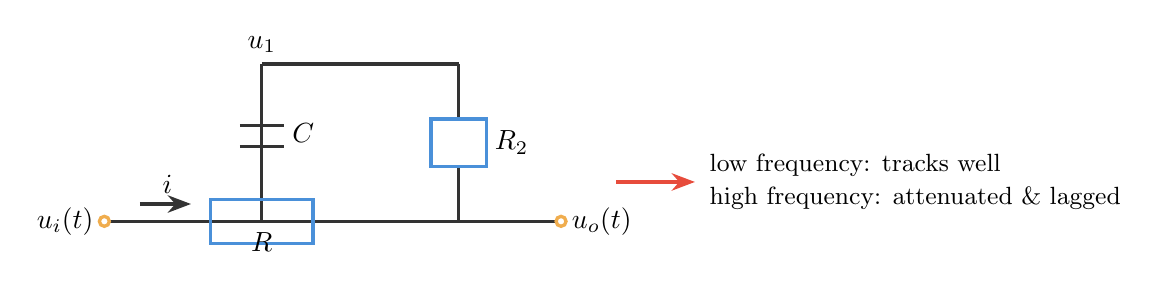
\begin{tikzpicture}[line width=1.2pt, >=Stealth]
  \draw[wiregray] (0,0) -- (1,0) -- (2.8,0) -- (5.8,0);
  \draw[wiregray] (2.0,0) -- (2.0,2.0);
  \draw[wiregray] (1.72,0.95) -- (2.28,0.95);
  \draw[wiregray] (1.72,1.22) -- (2.28,1.22);
  \draw[wiregray] (2.0,2.0) -- (4.5,2.0);
  \draw[wiregray] (4.5,2.0) -- (4.5,1.3);
  \draw[wiregray] (4.5,0.7) -- (4.5,0);
  \draw[blockblue] (1.35,-0.28) rectangle (2.65,0.28);
  \draw[blockblue] (4.15,0.7) rectangle (4.85,1.3);
  \filldraw[fill=white, draw=nodeorange] (0,0) circle (1.8pt);
  \filldraw[fill=white, draw=nodeorange] (5.8,0) circle (1.8pt);

  \node[left] at (0,0) {$u_i(t)$};
  \node[right] at (5.8,0) {$u_o(t)$};
  \node[below] at (2.0,0) {$R$};
  \node[right] at (4.82,1.0) {$R_2$};
  \node[right] at (2.25,1.12) {$C$};
  \node[above] at (2.0,2.0) {$u_1$};

  \draw[wiregray, ->] (0.45,0.22) -- (1.1,0.22);
  \node[above] at (0.8,0.22) {$i$};
  \draw[wiregray, ->, draw=sinkred] (6.5,0.5) -- (7.5,0.5);
  \node[right, align=left] at (7.55,0.5) {\small low frequency: tracks well\\\small high frequency: attenuated \& lagged};
\end{tikzpicture}
\end{document}
